% !TEX root = results_only.tex


describe the results generally

\section{Control case - uniform risk on a uniform population}

\begin{figure}[tb]
    \centering
    \begin{subfigure}[t]{0.45\textwidth}
    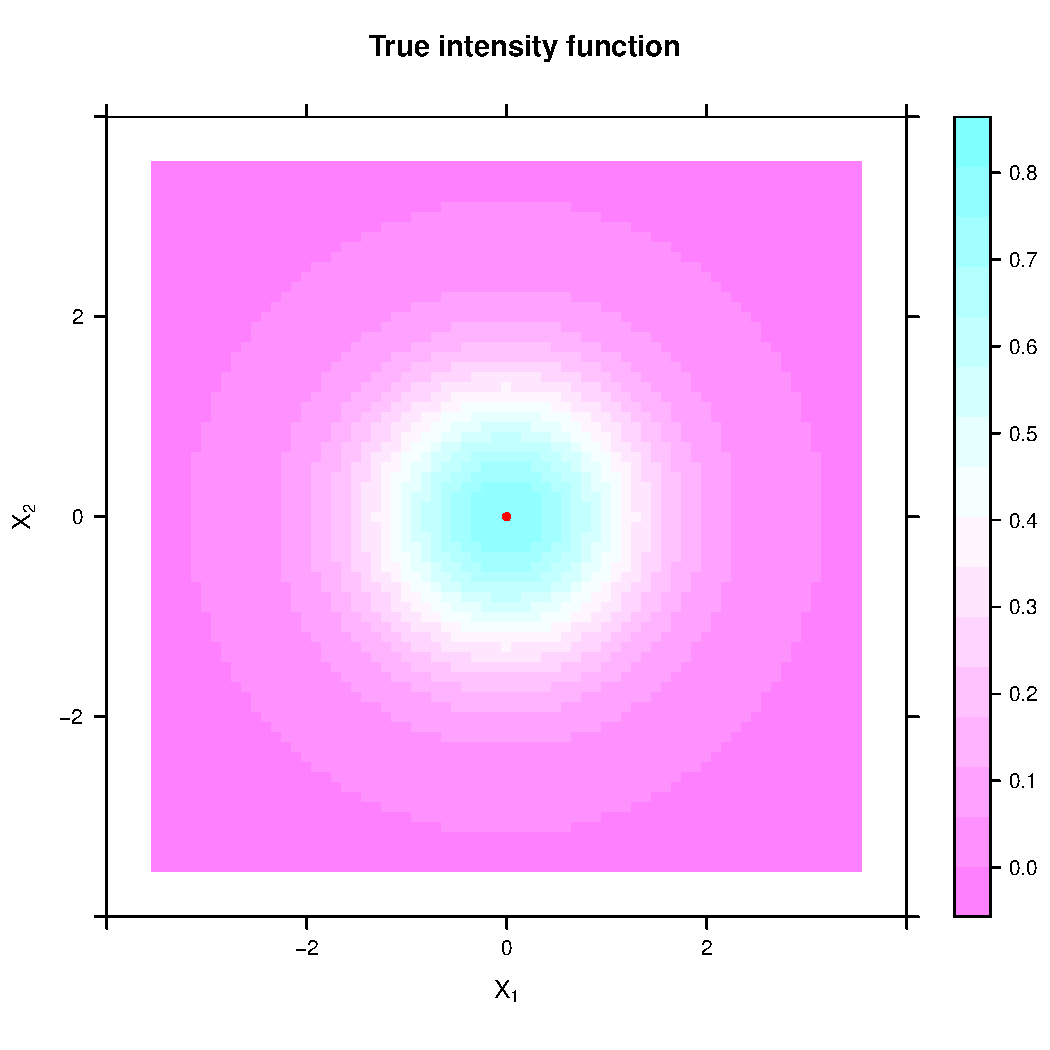
\includegraphics[width=\textwidth]{results/unif_100_1_unif/output/true_intensity_heatmap}
    \caption{True intensity}
    \end{subfigure}
    \begin{subfigure}[t]{0.45\textwidth}
    \includegraphics[width=\textwidth]{results/unif_100_1_unif/output/oracle_intensity_heatmap}
    \caption{Oracle estimate}
    \end{subfigure}
    \begin{subfigure}[b]{0.45\textwidth}
    \includegraphics[width=\textwidth]{results/unif_100_1_unif/output/silverman_intensity_heatmap}
    \caption{Silverman estimate}
    \end{subfigure}
    \begin{subfigure}[b]{0.45\textwidth}
    \includegraphics[width=\textwidth]{results/unif_100_1_unif/output/CV_intensity_heatmap}
    \caption{Cross-validation estimate}
    \end{subfigure}
    \label{fig:cases_unif_100_unif}
    \caption{Example cases: uniform intensity on uniform population, 100 cases}
\end{figure}

\begin{figure}[tb]
    \centering
    \begin{subfigure}[b]{0.45\textwidth}
    \includegraphics[width=\textwidth]{results/unif_100_1_unif/output/ise-relative-histogram}
    \caption{Relative ISE}
    \end{subfigure}
    \begin{subfigure}[b]{0.45\textwidth}
    \includegraphics[width=\textwidth]{results/unif_100_1_unif/output/ise-histogram}
    \caption{Absolute ISE}
    \end{subfigure}
    \caption[ISE: uniform on uniform]{Integrated squared error histogram for uniform intensity on a uniform population, 100 cases}
    \label{fig:ise_unif_100_1_unif}
\end{figure}

\section{Single-peak risk on a uniform population}
% latex table generated in R 3.4.0 by xtable 1.8-2 package
% Sat Aug  5 21:15:22 2017
\begin{tabular}{lrrr}
  \hline
 & Oracle & Silverman & CV \\ 
  \hline
MISE & 0.000022 & 0.000035 & 0.000034 \\ 
  Relative MISE & 0.003358 & 0.005293 & 0.005266 \\ 
  MIAE & 0.002505 & 0.003100 & 0.003092 \\ 
  Relative MIAE & 0.031010 & 0.038378 & 0.038279 \\ 
  Max Error & 0.020705 & 0.030617 & 0.030498 \\ 
  Peak bias & -0.012292 & 0.006167 & 0.006026 \\ 
  Relative Peak bias & -0.152166 & 0.076337 & 0.074592 \\ 
  Peak drift & 0.265067 & 0.409888 & 0.408051 \\ 
  Relative Peak drift & 0.037867 & 0.058555 & 0.058293 \\ 
  Centroid bias & -0.012639 & -0.000422 & -0.000492 \\ 
  Relative Centroid bias & -0.156464 & -0.005226 & -0.006090 \\ 
  Centroid drift & 0.199485 & 0.216521 & 0.216495 \\ 
  Relative Centroid drift & 0.028498 & 0.030932 & 0.030928 \\ 
   \hline
\end{tabular}


\section{Varying the number of cases}

\subsection{50 cases}
% latex table generated in R 3.4.0 by xtable 1.8-2 package
% Sat Aug  5 19:49:51 2017
\begin{table}[H]
\centering
\begin{tabular}{lrrr}
  \hline
 & Oracle & Silverman & CV \\ 
  \hline
MISE & 0.000008 & 0.000014 & 0.000014 \\ 
  Relative MISE & 0.005208 & 0.008600 & 0.008580 \\ 
  MIAE & 0.001568 & 0.001955 & 0.001953 \\ 
  Relative MIAE & 0.038833 & 0.048413 & 0.048363 \\ 
  Max Error & 0.012435 & 0.018787 & 0.018756 \\ 
  Peak bias & -0.007124 & 0.004056 & 0.004020 \\ 
  Relative Peak bias & -0.176378 & 0.100410 & 0.099522 \\ 
  Peak drift & 0.322404 & 0.476198 & 0.475222 \\ 
  Relative Peak drift & 0.046058 & 0.068028 & 0.067889 \\ 
  Centroid bias & -0.007304 & 0.000496 & 0.000487 \\ 
  Relative Centroid bias & -0.180839 & 0.012284 & 0.012057 \\ 
  Centroid drift & 0.262196 & 0.280772 & 0.281105 \\ 
  Relative Centroid drift & 0.037457 & 0.040110 & 0.040158 \\ 
   \hline
\end{tabular}
\caption{Mean error rates} 
\label{tbl:mean_error_rates}
\end{table}


\subsection{100 cases}
% latex table generated in R 3.4.0 by xtable 1.8-2 package
% Sat Aug  5 21:15:22 2017
\begin{tabular}{lrrr}
  \hline
 & Oracle & Silverman & CV \\ 
  \hline
MISE & 0.000022 & 0.000035 & 0.000034 \\ 
  Relative MISE & 0.003358 & 0.005293 & 0.005266 \\ 
  MIAE & 0.002505 & 0.003100 & 0.003092 \\ 
  Relative MIAE & 0.031010 & 0.038378 & 0.038279 \\ 
  Max Error & 0.020705 & 0.030617 & 0.030498 \\ 
  Peak bias & -0.012292 & 0.006167 & 0.006026 \\ 
  Relative Peak bias & -0.152166 & 0.076337 & 0.074592 \\ 
  Peak drift & 0.265067 & 0.409888 & 0.408051 \\ 
  Relative Peak drift & 0.037867 & 0.058555 & 0.058293 \\ 
  Centroid bias & -0.012639 & -0.000422 & -0.000492 \\ 
  Relative Centroid bias & -0.156464 & -0.005226 & -0.006090 \\ 
  Centroid drift & 0.199485 & 0.216521 & 0.216495 \\ 
  Relative Centroid drift & 0.028498 & 0.030932 & 0.030928 \\ 
   \hline
\end{tabular}


\subsection{200 cases}
% latex table generated in R 3.4.0 by xtable 1.8-2 package
% Sat Aug  5 21:44:37 2017
\begin{tabular}{lrrr}
  \hline
 & Oracle & Silverman & CV \\ 
  \hline
MISE & 0.000053 & 0.000083 & 0.000082 \\ 
  Relative MISE & 0.002029 & 0.003184 & 0.003129 \\ 
  MIAE & 0.003909 & 0.004852 & 0.004810 \\ 
  Relative MIAE & 0.024196 & 0.030032 & 0.029772 \\ 
  Max Error & 0.033936 & 0.049447 & 0.048810 \\ 
  Peak bias & -0.016473 & 0.010215 & 0.009458 \\ 
  Relative Peak bias & -0.101961 & 0.063224 & 0.058539 \\ 
  Peak drift & 0.219372 & 0.357137 & 0.353058 \\ 
  Relative Peak drift & 0.031339 & 0.051020 & 0.050437 \\ 
  Centroid bias & -0.017532 & -0.001587 & -0.001859 \\ 
  Relative Centroid bias & -0.108518 & -0.009821 & -0.011508 \\ 
  Centroid drift & 0.146327 & 0.158930 & 0.158287 \\ 
  Relative Centroid drift & 0.020904 & 0.022704 & 0.022612 \\ 
   \hline
\end{tabular}


\subsection{500 cases}
% latex table generated in R 3.4.0 by xtable 1.8-2 package
% Sat Aug  5 22:43:32 2017
\begin{tabular}{lrrr}
  \hline
 & Oracle & Silverman & CV \\ 
  \hline
MISE & 0.000170 & 0.000265 & 0.000244 \\ 
  Relative MISE & 0.001041 & 0.001626 & 0.001496 \\ 
  MIAE & 0.007096 & 0.008775 & 0.008421 \\ 
  Relative MIAE & 0.017567 & 0.021725 & 0.020849 \\ 
  Max Error & 0.065158 & 0.092681 & 0.087429 \\ 
  Peak bias & -0.023250 & 0.018688 & 0.012450 \\ 
  Relative Peak bias & -0.057562 & 0.046269 & 0.030824 \\ 
  Peak drift & 0.176919 & 0.293212 & 0.276800 \\ 
  Relative Peak drift & 0.025274 & 0.041887 & 0.039543 \\ 
  Centroid bias & -0.026539 & -0.003605 & -0.005705 \\ 
  Relative Centroid bias & -0.065707 & -0.008925 & -0.014124 \\ 
  Centroid drift & 0.096196 & 0.104184 & 0.103456 \\ 
  Relative Centroid drift & 0.013742 & 0.014883 & 0.014779 \\ 
   \hline
\end{tabular}


\subsection{1000 cases}
% latex table generated in R 3.4.0 by xtable 1.8-2 package
% Sun Aug  6 00:15:05 2017
\begin{table}[H]
\centering
\begin{tabular}{lrrr}
  \hline
 & Oracle & Silverman & CV \\ 
  \hline
MISE & 0.000379 & 0.000619 & 0.000484 \\ 
  Relative MISE & 0.000581 & 0.000948 & 0.000742 \\ 
  MIAE & 0.010804 & 0.013570 & 0.012061 \\ 
  Relative MIAE & 0.013375 & 0.016798 & 0.014931 \\ 
  Max Error & 0.105433 & 0.145677 & 0.126060 \\ 
  Peak bias & -0.034129 & 0.024518 & -0.000092 \\ 
  Relative Peak bias & -0.042248 & 0.030351 & -0.000114 \\ 
  Peak drift & 0.129044 & 0.251876 & 0.185739 \\ 
  Relative Peak drift & 0.018435 & 0.035982 & 0.026534 \\ 
  Centroid bias & -0.037516 & -0.001969 & -0.014152 \\ 
  Relative Centroid bias & -0.046441 & -0.002438 & -0.017519 \\ 
  Centroid drift & 0.068889 & 0.076451 & 0.074548 \\ 
  Relative Centroid drift & 0.009841 & 0.010922 & 0.010650 \\ 
   \hline
\end{tabular}
\caption{Mean error rates} 
\label{tbl:mean_error_rates}
\end{table}


\section{Varying the size of the population}

\subsection{100 cases from 10,000}
% latex table generated in R 3.4.0 by xtable 1.8-2 package
% Sat Aug  5 21:15:22 2017
\begin{tabular}{lrrr}
  \hline
 & Oracle & Silverman & CV \\ 
  \hline
MISE & 0.000022 & 0.000035 & 0.000034 \\ 
  Relative MISE & 0.003358 & 0.005293 & 0.005266 \\ 
  MIAE & 0.002505 & 0.003100 & 0.003092 \\ 
  Relative MIAE & 0.031010 & 0.038378 & 0.038279 \\ 
  Max Error & 0.020705 & 0.030617 & 0.030498 \\ 
  Peak bias & -0.012292 & 0.006167 & 0.006026 \\ 
  Relative Peak bias & -0.152166 & 0.076337 & 0.074592 \\ 
  Peak drift & 0.265067 & 0.409888 & 0.408051 \\ 
  Relative Peak drift & 0.037867 & 0.058555 & 0.058293 \\ 
  Centroid bias & -0.012639 & -0.000422 & -0.000492 \\ 
  Relative Centroid bias & -0.156464 & -0.005226 & -0.006090 \\ 
  Centroid drift & 0.199485 & 0.216521 & 0.216495 \\ 
  Relative Centroid drift & 0.028498 & 0.030932 & 0.030928 \\ 
   \hline
\end{tabular}


\subsection{1000 cases from 100,000}
% latex table generated in R 3.4.0 by xtable 1.8-2 package
% Sun Jul 30 00:05:45 2017
\begin{table}[ht]
\centering
\begin{tabular}{rrrr}
  \hline
 & Oracle & Silverman & CV \\ 
  \hline
MISE & 0.000002 & 0.000002 & 0.000002 \\ 
  Relative MISE & 0.000296 & 0.000275 & 0.000312 \\ 
  MIAE & 0.000172 & 0.000134 & 0.000169 \\ 
  Relative MIAE & 0.002123 & 0.001663 & 0.002093 \\ 
  Max Error & 0.003190 & 0.003425 & 0.003799 \\ 
  Peak bias & 0.004776 & 0.006378 & 0.006163 \\ 
  Relative Peak bias & 0.059119 & 0.078949 & 0.076294 \\ 
  Peak drift & 0.106483 & 0.145200 & 0.134117 \\ 
  Relative Peak drift & 0.015212 & 0.020743 & 0.019160 \\ 
  Centroid bias & 0.004937 & 0.007348 & 0.006476 \\ 
  Relative Centroid bias & 0.061119 & 0.090964 & 0.080164 \\ 
  Centroid drift & 0.059317 & 0.062619 & 0.061337 \\ 
  Relative Centroid drift & 0.008474 & 0.008946 & 0.008762 \\ 
   \hline
\end{tabular}
\caption{Standard deviation of error rates} 
\label{tbl:stddev_error_rates}
\end{table}


\section{Varying the decay of the risk function}

\subsection{100 cases with decay rate 0.5}
% latex table generated in R 3.4.0 by xtable 1.8-2 package
% Sat Aug  5 20:27:22 2017
\begin{table}[ht]
\centering
\begin{tabular}{rrrr}
  \hline
 & Oracle & Silverman & CV \\ 
  \hline
MISE & 0.000077 & 0.000131 & 0.000119 \\ 
  Relative MISE & 0.000734 & 0.001254 & 0.001144 \\ 
  MIAE & 0.002409 & 0.003038 & 0.002876 \\ 
  Relative MIAE & 0.007454 & 0.009399 & 0.008899 \\ 
  Max Error & 0.076835 & 0.117578 & 0.108564 \\ 
  Peak bias & -0.046725 & 0.020911 & 0.009059 \\ 
  Relative Peak bias & -0.144576 & 0.064704 & 0.028031 \\ 
  Peak drift & 0.129820 & 0.216138 & 0.203513 \\ 
  Relative Peak drift & 0.018546 & 0.030877 & 0.029073 \\ 
  Centroid bias & -0.054373 & -0.022933 & -0.029030 \\ 
  Relative Centroid bias & -0.168240 & -0.070958 & -0.089824 \\ 
  Centroid drift & 0.064940 & 0.071866 & 0.070546 \\ 
  Relative Centroid drift & 0.009277 & 0.010267 & 0.010078 \\ 
   \hline
\end{tabular}
\caption{Mean error rates} 
\label{tbl:mean_error_rates}
\end{table}


\subsection{100 cases with decay rate 0.7}
% latex table generated in R 3.4.2 by xtable 1.8-2 package
% Thu Dec  7 16:57:46 2017
\begin{tabular}{lrrr}
  \hline
 & Oracle & Silverman & CV \\ 
  \hline
MISE & 0.000042 & 0.000070 & 0.000067 \\ 
  Relative MISE & 0.001528 & 0.002568 & 0.002483 \\ 
  MIAE & 0.002425 & 0.003070 & 0.003019 \\ 
  Relative MIAE & 0.014713 & 0.018625 & 0.018318 \\ 
  Max Error & 0.041189 & 0.062268 & 0.060801 \\ 
  Peak bias & -0.020965 & 0.013460 & 0.011707 \\ 
  Relative Peak bias & -0.127194 & 0.081663 & 0.071024 \\ 
  Peak drift & 0.187770 & 0.306194 & 0.300844 \\ 
  Relative Peak drift & 0.026824 & 0.043742 & 0.042978 \\ 
  Centroid bias & -0.023222 & -0.008659 & -0.009076 \\ 
  Relative Centroid bias & -0.140888 & -0.052531 & -0.055064 \\ 
  Centroid drift & 0.114011 & 0.119838 & 0.119153 \\ 
  Relative Centroid drift & 0.016287 & 0.017120 & 0.017022 \\ 
   \hline
\end{tabular}


\subsection{100 cases with decay rate 1.0}
% latex table generated in R 3.4.0 by xtable 1.8-2 package
% Sat Aug  5 21:15:22 2017
\begin{tabular}{lrrr}
  \hline
 & Oracle & Silverman & CV \\ 
  \hline
MISE & 0.000022 & 0.000035 & 0.000034 \\ 
  Relative MISE & 0.003358 & 0.005293 & 0.005266 \\ 
  MIAE & 0.002505 & 0.003100 & 0.003092 \\ 
  Relative MIAE & 0.031010 & 0.038378 & 0.038279 \\ 
  Max Error & 0.020705 & 0.030617 & 0.030498 \\ 
  Peak bias & -0.012292 & 0.006167 & 0.006026 \\ 
  Relative Peak bias & -0.152166 & 0.076337 & 0.074592 \\ 
  Peak drift & 0.265067 & 0.409888 & 0.408051 \\ 
  Relative Peak drift & 0.037867 & 0.058555 & 0.058293 \\ 
  Centroid bias & -0.012639 & -0.000422 & -0.000492 \\ 
  Relative Centroid bias & -0.156464 & -0.005226 & -0.006090 \\ 
  Centroid drift & 0.199485 & 0.216521 & 0.216495 \\ 
  Relative Centroid drift & 0.028498 & 0.030932 & 0.030928 \\ 
   \hline
\end{tabular}


\subsection{100 cases with decay rate 1.4}
% latex table generated in R 3.4.2 by xtable 1.8-2 package
% Thu Dec  7 17:09:22 2017
\begin{tabular}{lrrr}
  \hline
 & Oracle & Silverman & CV \\ 
  \hline
MISE & 0.000012 & 0.000019 & 0.000019 \\ 
  Relative MISE & 0.006627 & 0.010652 & 0.010635 \\ 
  MIAE & 0.002291 & 0.002949 & 0.002946 \\ 
  Relative MIAE & 0.054683 & 0.070397 & 0.070338 \\ 
  Max Error & 0.011293 & 0.016460 & 0.016441 \\ 
  Peak bias & -0.005739 & 0.003331 & 0.003308 \\ 
  Relative Peak bias & -0.137007 & 0.079526 & 0.078980 \\ 
  Peak drift & 0.407527 & 0.576641 & 0.576732 \\ 
  Relative Peak drift & 0.058218 & 0.082377 & 0.082390 \\ 
  Centroid bias & -0.005876 & 0.001197 & 0.001182 \\ 
  Relative Centroid bias & -0.140265 & 0.028578 & 0.028217 \\ 
  Centroid drift & 0.337723 & 0.384568 & 0.383883 \\ 
  Relative Centroid drift & 0.048246 & 0.054938 & 0.054840 \\ 
   \hline
\end{tabular}


\subsection{100 cases with decay rate 2.0}
% latex table generated in R 3.4.0 by xtable 1.8-2 package
% Sat Aug  5 21:31:40 2017
\begin{table}[ht]
\centering
\begin{tabular}{lrrr}
  \hline
 & Oracle & Silverman & CV \\ 
  \hline
MISE & 0.000006 & 0.000012 & 0.000012 \\ 
  Relative MISE & 0.011308 & 0.021333 & 0.021316 \\ 
  MIAE & 0.001867 & 0.002638 & 0.002637 \\ 
  Relative MIAE & 0.079514 & 0.112328 & 0.112282 \\ 
  Max Error & 0.006153 & 0.010407 & 0.010401 \\ 
  Peak bias & -0.003225 & 0.003258 & 0.003251 \\ 
  Relative Peak bias & -0.137322 & 0.138713 & 0.138426 \\ 
  Peak drift & 0.615800 & 0.900437 & 0.900381 \\ 
  Relative Peak drift & 0.087971 & 0.128634 & 0.128626 \\ 
  Centroid bias & -0.003271 & 0.001927 & 0.001923 \\ 
  Relative Centroid bias & -0.139292 & 0.082052 & 0.081892 \\ 
  Centroid drift & 0.534199 & 0.668770 & 0.668461 \\ 
  Relative Centroid drift & 0.076314 & 0.095539 & 0.095494 \\ 
   \hline
\end{tabular}
\caption{Mean error rates} 
\label{tbl:mean_error_rates}
\end{table}


\section{Varying the decay of the population density}

\subsection{100 cases with uniform population}
% latex table generated in R 3.4.0 by xtable 1.8-2 package
% Sat Aug  5 21:15:22 2017
\begin{tabular}{lrrr}
  \hline
 & Oracle & Silverman & CV \\ 
  \hline
MISE & 0.000022 & 0.000035 & 0.000034 \\ 
  Relative MISE & 0.003358 & 0.005293 & 0.005266 \\ 
  MIAE & 0.002505 & 0.003100 & 0.003092 \\ 
  Relative MIAE & 0.031010 & 0.038378 & 0.038279 \\ 
  Max Error & 0.020705 & 0.030617 & 0.030498 \\ 
  Peak bias & -0.012292 & 0.006167 & 0.006026 \\ 
  Relative Peak bias & -0.152166 & 0.076337 & 0.074592 \\ 
  Peak drift & 0.265067 & 0.409888 & 0.408051 \\ 
  Relative Peak drift & 0.037867 & 0.058555 & 0.058293 \\ 
  Centroid bias & -0.012639 & -0.000422 & -0.000492 \\ 
  Relative Centroid bias & -0.156464 & -0.005226 & -0.006090 \\ 
  Centroid drift & 0.199485 & 0.216521 & 0.216495 \\ 
  Relative Centroid drift & 0.028498 & 0.030932 & 0.030928 \\ 
   \hline
\end{tabular}


\subsection{100 cases with population decay rate 2.0}
% latex table generated in R 3.4.0 by xtable 1.8-2 package
% Sat Aug  5 21:07:06 2017
\begin{table}[H]
\centering
\begin{tabular}{lrrr}
  \hline
 & Oracle & Silverman & CV \\ 
  \hline
MISE & 0.000021 & 0.000034 & 0.000034 \\ 
  Relative MISE & 0.003273 & 0.005274 & 0.005179 \\ 
  MIAE & 0.002642 & 0.003221 & 0.003194 \\ 
  Relative MIAE & 0.032700 & 0.039874 & 0.039542 \\ 
  Max Error & 0.020044 & 0.030183 & 0.029789 \\ 
  Peak bias & -0.009647 & 0.006342 & 0.005880 \\ 
  Relative Peak bias & -0.119422 & 0.078502 & 0.072792 \\ 
  Peak drift & 0.309850 & 0.468400 & 0.464955 \\ 
  Relative Peak drift & 0.044264 & 0.066914 & 0.066422 \\ 
  Centroid bias & -0.010650 & -0.004896 & -0.004979 \\ 
  Relative Centroid bias & -0.131838 & -0.060607 & -0.061636 \\ 
  Centroid drift & 0.192663 & 0.192580 & 0.192641 \\ 
  Relative Centroid drift & 0.027523 & 0.027511 & 0.027520 \\ 
   \hline
\end{tabular}
\caption{Mean error rates} 
\label{tbl:mean_error_rates}
\end{table}


\subsection{100 cases with population decay rate 1.4}
% latex table generated in R 3.4.0 by xtable 1.8-2 package
% Sat Aug  5 21:37:13 2017
\begin{table}[ht]
\centering
\begin{tabular}{rrrr}
  \hline
 & Oracle & Silverman & CV \\ 
  \hline
MISE & 0.000023 & 0.000036 & 0.000034 \\ 
  Relative MISE & 0.003558 & 0.005476 & 0.005188 \\ 
  MIAE & 0.002836 & 0.003304 & 0.003227 \\ 
  Relative MIAE & 0.035109 & 0.040906 & 0.039946 \\ 
  Max Error & 0.019837 & 0.031477 & 0.030030 \\ 
  Peak bias & -0.008783 & 0.006794 & 0.005493 \\ 
  Relative Peak bias & -0.108731 & 0.084104 & 0.067997 \\ 
  Peak drift & 0.279824 & 0.422472 & 0.412451 \\ 
  Relative Peak drift & 0.039975 & 0.060353 & 0.058922 \\ 
  Centroid bias & -0.009989 & -0.004347 & -0.004578 \\ 
  Relative Centroid bias & -0.123654 & -0.053816 & -0.056672 \\ 
  Centroid drift & 0.154247 & 0.149632 & 0.149878 \\ 
  Relative Centroid drift & 0.022035 & 0.021376 & 0.021411 \\ 
   \hline
\end{tabular}
\caption{Mean error rates} 
\label{tbl:mean_error_rates}
\end{table}


\subsection{100 cases with population decay rate 1.0}
% latex table generated in R 3.4.0 by xtable 1.8-2 package
% Sat Aug  5 23:00:37 2017
\begin{table}[ht]
\centering
\begin{tabular}{rrrr}
  \hline
 & Oracle & Silverman & CV \\ 
  \hline
MISE & 0.000066 & 0.000087 & 0.000078 \\ 
  Relative MISE & 0.010123 & 0.013299 & 0.011878 \\ 
  MIAE & 0.003812 & 0.004124 & 0.003938 \\ 
  Relative MIAE & 0.047184 & 0.051056 & 0.048743 \\ 
  Max Error & 0.054969 & 0.086132 & 0.074745 \\ 
  Peak bias & 0.002495 & 0.028003 & 0.019537 \\ 
  Relative Peak bias & 0.030881 & 0.346652 & 0.241856 \\ 
  Peak drift & 0.875427 & 1.234994 & 1.090434 \\ 
  Relative Peak drift & 0.125061 & 0.176428 & 0.155776 \\ 
  Centroid bias & -0.011069 & -0.005650 & -0.006984 \\ 
  Relative Centroid bias & -0.137022 & -0.069944 & -0.086449 \\ 
  Centroid drift & 0.238070 & 0.225614 & 0.227857 \\ 
  Relative Centroid drift & 0.034010 & 0.032231 & 0.032551 \\ 
   \hline
\end{tabular}
\caption{Mean error rates} 
\label{tbl:mean_error_rates}
\end{table}


\subsection{100 cases with population decay rate 0.7}
% latex table generated in R 3.3.3 by xtable 1.8-2 package
% Mon Jan 15 21:47:29 2018
\begin{tabular}{lrrr}
  \hline
 & Oracle & Silverman & CV \\ 
  \hline
MISE & 0.000022 & 0.000035 & 0.000033 \\ 
  Relative MISE & 0.003402 & 0.005404 & 0.004996 \\ 
  Normalized MISE & 0.000022 & 0.000035 & 0.000033 \\ 
  MIAE & 0.002515 & 0.003126 & 0.003003 \\ 
  Relative MIAE & 0.031137 & 0.038695 & 0.037178 \\ 
  Max Error & 0.021087 & 0.031111 & 0.029319 \\ 
  Peak bias & -0.010671 & 0.006739 & 0.004427 \\ 
  Relative Peak bias & -0.132093 & 0.083426 & 0.054803 \\ 
  Peak drift & 0.288634 & 0.418493 & 0.401299 \\ 
  Relative Peak drift & 0.041233 & 0.059785 & 0.057328 \\ 
  Centroid bias & -0.011216 & -0.000155 & -0.001331 \\ 
  Relative Centroid bias & -0.138849 & -0.001917 & -0.016472 \\ 
  Centroid drift & 0.207657 & 0.222708 & 0.221023 \\ 
  Relative Centroid drift & 0.029665 & 0.031815 & 0.031575 \\ 
   \hline
\end{tabular}


\section{Varying the distance between two peaks}

\subsection{100 cases in 2 peaks separated by 1}
% latex table generated in R 3.3.3 by xtable 1.8-2 package
% Sun Mar 11 18:25:14 2018
\begin{tabular}{lrrr}
  \hline
 & Oracle & Silverman & CV \\ 
  \hline
MISE & 0.000020 & 0.000028 & 0.000028 \\ 
  Relative MISE & 0.003806 & 0.005434 & 0.005499 \\ 
  Normalized MISE & 0.000000 & 0.000000 & 0.000000 \\ 
  MIAE & 0.002482 & 0.002946 & 0.002911 \\ 
  Relative MIAE & 0.034598 & 0.041069 & 0.040574 \\ 
  Normalized MIAE & 0.000000 & 0.000000 & 0.000000 \\ 
  Max Error & 0.018613 & 0.025324 & 0.024450 \\ 
  Normalized Max Error & 0.000002 & 0.000003 & 0.000002 \\ 
  Peak bias & -0.008775 & 0.002958 & -0.002987 \\ 
  Relative Peak bias & -0.122312 & 0.041234 & -0.041636 \\ 
  Peak drift & 0.308419 & 0.424717 & 0.350763 \\ 
  Relative Peak drift & 0.044060 & 0.060674 & 0.050109 \\ 
  Centroid bias & -0.009281 & -0.001295 & -0.007951 \\ 
  Relative Centroid bias & -0.129358 & -0.018055 & -0.110820 \\ 
  Centroid drift & 0.225096 & 0.241028 & 0.222905 \\ 
  Relative Centroid drift & 0.032157 & 0.034433 & 0.031844 \\ 
   \hline
\end{tabular}


\subsection{100 cases in 2 peaks separated by 2}
% latex table generated in R 3.4.0 by xtable 1.8-2 package
% Sat Aug  5 21:30:32 2017
\begin{table}[ht]
\centering
\begin{tabular}{rrrr}
  \hline
 & Oracle & Silverman & CV \\ 
  \hline
MISE & 0.000016 & 0.000020 & 0.000020 \\ 
  Relative MISE & 0.005500 & 0.006847 & 0.006843 \\ 
  MIAE & 0.002450 & 0.002728 & 0.002727 \\ 
  Relative MIAE & 0.045229 & 0.050364 & 0.050348 \\ 
  Max Error & 0.015217 & 0.018315 & 0.018306 \\ 
  Peak bias & -0.007724 & -0.000374 & -0.000390 \\ 
  Relative Peak bias & -0.142615 & -0.006911 & -0.007195 \\ 
  Peak drift & 0.446284 & 0.521588 & 0.521333 \\ 
  Relative Peak drift & 0.063755 & 0.074513 & 0.074476 \\ 
  Centroid bias & -0.007922 & -0.002078 & -0.002088 \\ 
  Relative Centroid bias & -0.146276 & -0.038374 & -0.038550 \\ 
  Centroid drift & 0.425758 & 0.425942 & 0.425824 \\ 
  Relative Centroid drift & 0.060823 & 0.060849 & 0.060832 \\ 
   \hline
\end{tabular}
\caption{Mean error rates} 
\label{tbl:mean_error_rates}
\end{table}


\subsection{100 cases in 2 peaks separated by 3}
% latex table generated in R 3.4.0 by xtable 1.8-2 package
% Sat Aug  5 21:31:15 2017
\begin{table}[ht]
\centering
\begin{tabular}{lrrr}
  \hline
 & Oracle & Silverman & CV \\ 
  \hline
MISE & 0.000018 & 0.000019 & 0.000019 \\ 
  Relative MISE & 0.007368 & 0.007591 & 0.007591 \\ 
  MIAE & 0.002675 & 0.002735 & 0.002735 \\ 
  Relative MIAE & 0.053776 & 0.054989 & 0.054991 \\ 
  Max Error & 0.016647 & 0.016798 & 0.016799 \\ 
  Peak bias & -0.010884 & -0.010384 & -0.010381 \\ 
  Relative Peak bias & -0.218843 & -0.208792 & -0.208735 \\ 
  Peak drift & 0.550466 & 0.541528 & 0.541476 \\ 
  Relative Peak drift & 0.078638 & 0.077361 & 0.077354 \\ 
  Centroid bias & -0.011999 & -0.011748 & -0.011746 \\ 
  Relative Centroid bias & -0.241255 & -0.236209 & -0.236168 \\ 
  Centroid drift & 0.581652 & 0.562239 & 0.562221 \\ 
  Relative Centroid drift & 0.083093 & 0.080320 & 0.080317 \\ 
   \hline
\end{tabular}
\caption{Mean error rates} 
\label{tbl:mean_error_rates}
\end{table}


\subsection{100 cases in 2 peaks separated by 4}
% latex table generated in R 3.4.2 by xtable 1.8-2 package
% Sat Feb 17 16:40:52 2018
\begin{tabular}{lrrr}
  \hline
 & Oracle & Silverman & CV \\ 
  \hline
MISE & 0.000020 & 0.000024 & 0.000022 \\ 
  Relative MISE & 0.007604 & 0.009208 & 0.008191 \\ 
  Normalized MISE & 0.000020 & 0.000024 & 0.000022 \\ 
  MIAE & 0.002820 & 0.003099 & 0.002921 \\ 
  Relative MIAE & 0.054779 & 0.060198 & 0.056745 \\ 
  Max Error & 0.017580 & 0.019430 & 0.018238 \\ 
  Peak bias & -0.011073 & -0.017197 & -0.011963 \\ 
  Relative Peak bias & -0.215103 & -0.334060 & -0.232374 \\ 
  Peak drift & 0.641297 & 0.420580 & 0.595129 \\ 
  Relative Peak drift & 0.091614 & 0.060083 & 0.085018 \\ 
  Centroid bias & -0.015923 & -0.019127 & -0.016312 \\ 
  Relative Centroid bias & -0.309304 & -0.371538 & -0.316860 \\ 
  Centroid drift & 0.644231 & 0.502452 & 0.625179 \\ 
  Relative Centroid drift & 0.092033 & 0.071779 & 0.089311 \\ 
   \hline
\end{tabular}



